\documentclass[course=asp]{aspdoc}
\usepackage{graphicx}
\graphicspath{{./Bilder/}}

\newcommand{\theGroup}{team 117} % Beispiel: 42
\newcommand{\theNumber}{502: XTEA} 
\author{Guo, Linfeng\\Gönenc, Hazar \\Özakay, Baris}
\date{Wintersemester 2021/22} 


% Diese Zeile bitte -nicht- aendern.
\title{Gruppe \theGroup{} -- Abgabe zu Aufgabe \theNumber}

\begin{document}
\maketitle



\section{Einleitung}
Im Rahmen unseres Projektes im Fach Aspekte der systemnahen Programmierung bei der Spieleentwicklung war es unsere Aufgabe, ein Ver- und Entschlüsselungsalgorithmus XTea in Assemblercode zu programmieren. Diese Aufgabe lässt sich in folgende Bereiche aufteilen: Konzeption, die Funktionsweise des XTEA Algorithmus und Verfahren für die Optimierung des Algorithmus, verstehen; der XTEA Algorithmus in Assemblercode zu implementieren …(Aufgabe von Baris). Die Bearbeitung dieser Teilbereiche wird im Folgenden Beschrieben.  \\In der Grafik zu sehen ist ein Beispiel für die Ver- und Entschlüsselung mit dem XTEA Algorithmus.  

\newpage
\section{Lösungsansatz}
\subsection*{2.1.Feistelchiffre }
Der XTEA Algorithmus ist ein Verschlüsselungsalgorithmus, welche auf die Struktur von Feistelchiffre basiert ist. Feistelchiffre ist eine Struktur, die für symmetrische Verschlüsselung verwendet wird. Unter symmetrische Verschlüsselung ist zu verstehen, dass für die Ver- und Entschlüsselung nur ein Key verwendet wird. Wir würden daher erstmal mit Feistelchiffre, die grundstruktur der symmetrische Verschlüsselung, eingehen.\\
Feistelchiffre lässt sich in vier Schritten aufteilen. Zuerst hat man ein Klartextblock mit der Nachricht, weche meist 8 Bytes ist, und teilt diese in zwei gleich große Bl\"ocke L0 und R0, die 4 Bytes entsprechen auf.

\begin{table}[H]
\centering 
    \begin{tabular}{|l|l|l|l|l|l|l|l|}
        \hline
        B & E & I & S & P & I & E & L   \\
        \hline
    \end{tabular}
    \caption{Nachricht}
\end{table}

\begin{table}[H]
\centering 
    \begin{tabular}{|l|l|l|l|l|l|l|l|}
        \hline
        42 & 45 & 49 & 53 & 50 & 49 & 25 & 4C   \\
        \hline
    \end{tabular}
    \caption{Nachricht in Hex Code}
\end{table}



\begin{table}[H]
    
    \begin{minipage}{.5\linewidth}
      
      \centering
        \begin{tabular}{|l|l|l|l|}
		\hline
            42 & 45 & 49 & 53   \\
		\hline
        \end{tabular}

	\caption{L0}
    \end{minipage}%
    \begin{minipage}{.5\linewidth}
    
 \centering
        
        \begin{tabular}{|l|l|l|l|}
           \hline
		 50 & 49 & 25 & 4C   \\
		\hline
        \end{tabular}
\caption{R0} 
    \end{minipage}
\end{table}
Danach findet die eigentliche Verschlüsselung statt. Man führt die Verschlüsselungsfunktion mit der Schlüssel,der ebenfalls 4 Byte entspricht, auf R0 aus. Die Funktion bei Feistelchiffre ist allerdings undefiniert, da Feistelchiffre nur die Struktur anbietet. Der Wert der durch die Funktion ergibt, wird anschließend mit dem linken Teil durch die XOR- Operation eingefangen. So ergibt sich das neue R1. Die ursprüngliche R0 wird dann zu L1. Nach jeder Verschlüsselung wird die Position vom linken und dem rechten Block getauscht, sowie oben beschrieben wird.\\
Die Entschlüsselung funktioniert im Prinzip genau wie die Verschlüsselung. Nur mit dem Unterschied, dass man die Position vom linken und rechten Teil tauscht. Also wird Ln+1 in die Funktion mit demselben Key eingesetzt und das Ergebnis wird dann mit Rn+1 per XOR abgebildet. Der Wert wird dann zu Rn und Ln+1 wird zu Ln.  


\begin{figure}[h]
\centering
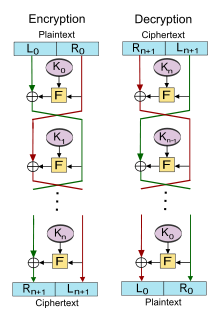
\includegraphics{Feistelchiffre.png}
\caption{Feistelchiffre}
\end{figure}
\newpage




\subsection*{2.2.XTEA}
\newpage
\subsection*{2.3.Padding}

%%test
\newpage
% TODO: Je nach Aufgabenstellung einen der Begriffe wählen
\section{Korrektheit/Genauigkeit}
\subsection*{I/O-Operationen in C}
\subsection*{Implementierung in C}
\subsection*{Implementierung in Assemblercode}
\newpage

\section{Performanzanalyse}
\newpage

\section{Zusammenfassung und Ausblick}

\newpage
% TODO: Fuegen Sie Ihre Quellen der Datei Ausarbeitung.bib hinzu
% Referenzieren Sie diese dann mit \cite{}.
% Beispiel: CR2 ist ein Register der x86-Architektur~\cite{intel2017man}.

%%TODO
\bibliographystyle{plain}
\bibliography{Ausarbeitung}{}

\end{document}
